%!TEX root = ../main.tex
%TODO: Redo the flowchart with updated and more specific steps

This chapter covers the steps needed to produce the wanted results. The input needed is a fiducial marker $M$ to provide the object position in the real world; and a 3D mesh $O$ which will be rendered in Augmented Reality. The output is a set of light sources $L_i$, each one having a position, orientation, intensity, color, type and size. In order to complete the luminance ($L()$) analysis a 360 panoramic image is required, but it will be generated in a previous step with a separate application as explained in the Theoretical Framework chapter. The entirety of the process is layed out in the flowchart in Figure 1, and each step is described in more detail afterwards.

\begin{figure}[H]
  \centering
  \setlength{\unitlength}{\textwidth} 
    \begin{picture}(1,0.5)
       \put(-0.1,0){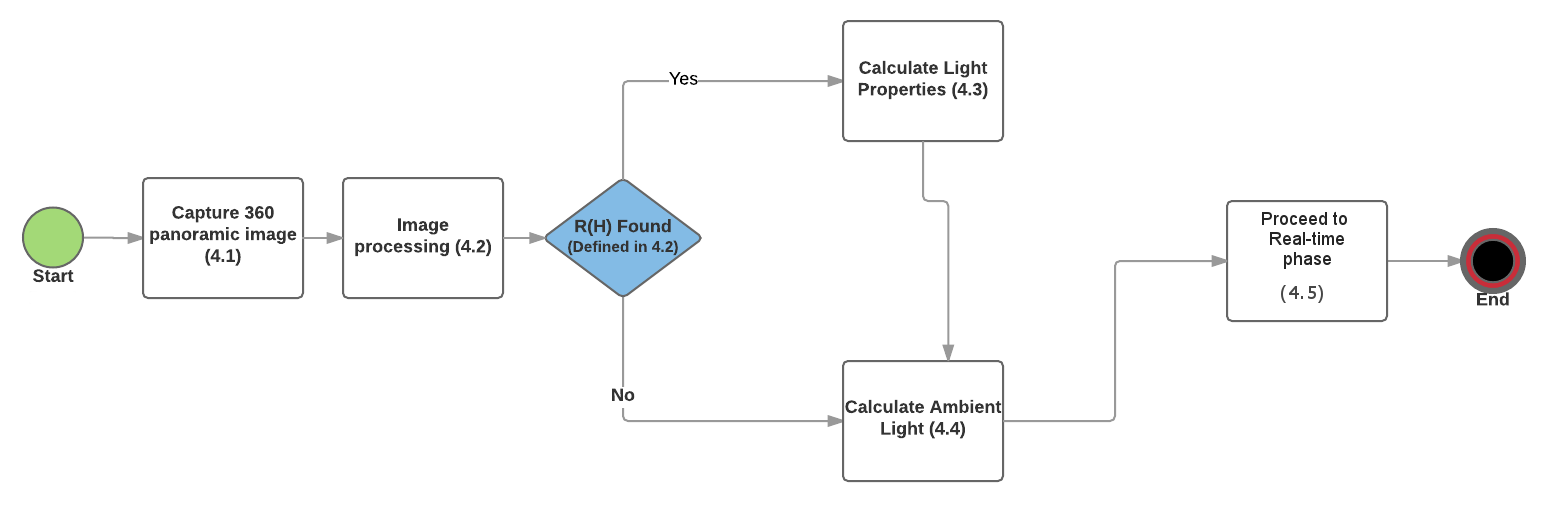
\includegraphics[width=1.3\unitlength]{Figures/Flowchart.png}}
       
    \end{picture}
    \caption{The method in a nutshell}
\end{figure}

\section{Capture 360 panoramic image}
In this work panoramic images are used as a tool, therefore it's not within the scope of the method to define a new way of capturing 360 images. The suggested application to procure a spherical panoramic image within the device itself is Google Street View.
The origin of the virtual world for placing and orienting $O$ within it is asked to the user by rotating the virtual reflective sphere so that the texture offset matches the device orientation within the real world. This will also simplify calculations of light orientations later on.

\section{Image processing}
Once the panoramic image is loaded and oriented the first step in order to be able to analyze the luminance is to get rid of the chromatic information. This is achieved with the following equation:

\begin{equation}
    L(R_{ij},G_{ij},B_{ij}) = 0,2126 \times R_{ij} + 0,7152 \times G_{ij} + 0,0722 \times B_{ij}; \quad \forall \  P_{ij}
\end{equation}

Where $L$ is the luminance obtained at D65 white point and $P$ is the pixel in the $i,j$ position of the image \newline
The contrast ratio has to be adjusted, so that the regions with high luminance are more clearly differentiable. 

\begin{equation}
     g(i,j) = \alpha \times f(i,j) + \beta
\end{equation}

Where $g(i,j)$ is the adjusted image, $f(i,j)$ is the original grayscale image and $\alpha$ and $\beta$ are the brightness and contrast constants, determined by parameter tuning. The parameter tuning will be carried out in a trial and error way, propose initial extreme values and run the program, changing the values in order to achieve the best result. The values that worked in the implementation were $\alpha = 220$ and $\beta = 255$.
In order to prevent outlier pixels and noise from causing false positives, let $g(i,j)$ be normalized like so:

\begin{equation}
    L(P_{ij}) = \frac{ 2 \times P_{ij} }{min(L) + max(L)}
\end{equation}

Where $min(L)$ and $max(L)$ are the overall minimum and maximum luminance values in the image. 
\newline
The result of these steps is a black and white image with the rough shape of the light source. If the image ends up completely black it means there are no important visible light sources and ambient illumination alone would give a good enough result on the rendered model. A region of high luminance is defined as follows:

\begin{equation}
    R(H) = \{p_{00}, p_{01}, ... , p_{mn}\}
\end{equation}
 Where $p_{ij}$ is the pixel in the i,j position of the image. Such that 
\[
    L(p_{ij}) > 0.9 \times max(L(p_{ij})) 
\]

The region must also be continuous, so the pixels must be adjacent.\newline
If there are regions of high luminance in the image, they would be discovered with a fair amount of noise and artifacts, caused by clear objects, reflections of light sources on highly reflective surfaces, or even light sources that are so far away in the distance that don't really contribute an important amount of light to the area of interest. Therefore it's necessary to also add a relative size constraint to the definition. What constitutes an acceptable region size to deem the light source is not an easy question to answer. The best approach to face this problem is to define it as a percentage of the width and height of the overall image and tune the parameter in search for the best solution. The size constraint would therefore be:

\begin{equation}
    width(R(H)) \times height(R(H)) \geq k \times W \times H
\end{equation}

Where $k$ is the parameter to be tuned, in the implementation the value that yielded the best results was $k = 0.004$; $W$ and $H$ are the total image width and height.\newline

These constraints also help keep the amount of lights to be processed within an acceptable range for a real-time application, even if the real environment has many light sources a simplification of them is necessary when modelling them to keep the application feasible. In the implementation the maximum amount of lights was capped to 8 because the overall performance of the application started to suffer with more lights. However, in order to identify the most relevant light sources it's necessary to calculate their parameters first.\newline
Once a set of light sources have been identified their properties need to be calculated.

\section{Calculate light properties}
The properties needed to calculate for each light are orientation, intensity and color. In the real world it is not trivial to calculate the position from just a single point of view as input, so even though the simulation would be a lot more robust if the actual position with respect to the camera was simulated there is just not enough information to calculate it in this method and all the lights are assumed to be at unit distance from the camera. With this in mind, all the other properties can be calculated.

\begin{enumerate}
\item Position:The x, y and z components will be those of the unit orientation vector, to ensure that the light is in the correct direction at unit distance.

\item  Orientation: The pixel coordinates (x,y) of the centroid of each light within the luminance panorama are saved. The image is projected on a sphere. The camera casts rays onto the sphere from 4 different points of view, 0\degree , 90\degree, 180\degree  and 270\degree. If the ray hits a white pixel and the pixel coordinates of the hit are approximately those of the centroid the light direction is calculated as follows:
\begin{equation}
    O(L_p) = -2 \times (N_h \cdot C_r) N_h + C_r
\end{equation}
Where $O(L_p)$ is the orientation of the pth light source, $N_h$ is the sphere normal on the hit point, $C_r$ and is the camera ray direction.
\item Color: Storing both versions of the panorama, one in full color and another one after processing will allow us to have both the color and the luminance information. Once a light source is detected, the equivalent area in the color image can be averaged to determine the color of the light source.
\item Intensity: There are two factors that influence the intensity of a light as perceived by a camera, the light size and the color temperature. The light's color temperature in Kelvin can be calculated as follows:
\begin{equation}
    T(C_p) = -949.86315 + 6253.80338 ^ {\frac{-n}{0.92159} } + 28.70599 ^{\frac{-n}{0.20039} } + 0.00004 ^ {\frac{-n}{0.07125} }
\end{equation}
\begin{equation}
n = {\frac{0.23881\times R + 0.25449\times G - 0.58291\times B}{0.11109\times R - 0.85406\times G + 0.52289\times B} }
\end{equation}

Where $R, G, B$ are the red, green and blue components of the light color.\newline 
The size analogy is given by the integral of the region of high luminance with respect to the full image. The light intensity is finally expressed by:
\begin{equation}
I(L_p) = T(C_p) \times \int_R L(i) \,dx
\end{equation}
Where $L(i)$ is the output image of the luminance analysis and $R$ is the pth region of high luminance.\newline 

\end{enumerate}

\section{Calculate ambient light}
Environment mapping is an image-based technique to approximate the appearance of the overall light conditions of an environment. This is accomplished by means of a precomputed texture image mapped as a far-away environment surrounding. Said surrounding is usually a geometric surface, when Blinn first introduced the method\cite{Blinn76} a sphere was used. Nowadays there are other alternatives, such as cube, paraboloid, pyramid or cylinder maps. The principle for each surface is the same, but the way to map a planar image onto the surface varies per surface.\newline
Since a panoramic image of the environment is already available using it to implement environment mapping would be an adequate use of resources. In order to generate an environment map it is necessary that the panorama is made into a High Dynamic Range image. This is because the Low Dynamic Range image captured directly from the device camera fails to capture the information necessary to simulate correct color balance, shadows, and highlights of the lighting environment; ultimately producing both inaccurate and less visually pleasing results. This has been illustrated by Paul Debevec.\cite{DebevecRSO}\newline 
A relatively easy and effective way to make an image into an HDR version is a technique called Tone Mapping, in which versions with different exposure values of the same image are blended together to include the full range of highlights and shadows of the overexposed and underexposed versions in a single image. Since asking the user to capture the environment more than once would have a bad impact on user friendliness, and also it's highly unlikely that the produced image would have the exact same framing every time, the different exposure values for the Tone Mapping will be produced altering the brightness and contrast values of the base image using equation 2 once again. After that the HDR image is produced using Debevec's weighting algorithm\cite{Debevec}.\newline
It's important to disclaim that the Tone Mapping process will not yield an actual HDR image. In the first place, it will be a standard 24 bit image in the $0...255$ range, with highlight and shadow valued clipped. The upside to still going through this process nonetheless is that the environment will be described in a richer way, capturing the bright areas and the shadows better than the standard exposure image.\newline
After the HDR version of the panorama is created it can be used to have an actual ground truth about the environment light color and intensity at any given point in the virtual space. This will be detailed in the Real-time Phase step subsection.

\section{Real-time Phase}
The original sphere panoramic photograph is widely used in the real time phase. It is used to create a cubemap of the real environment to be used as ambient lighting, to calculate the ambient contribution of the diffuse shaders and to fake reflections for the specular shaders.
\begin{enumerate}

\item Cubemap: The image coordinates are first converted to polar and divided into four regions by latitude $-\Pi/4 < \theta < \Pi/4 , \Pi/4 < \theta < 3\Pi/4, 3\Pi/4 < \theta < 5\Pi/4, 5\Pi/4 < \theta < 7\Pi/4$. These represent either one of the four faces of the cube, top or bottom. The projected coordinate is given by:
\begin{equation}
P = (1, tan(\phi), \frac{cot(\theta)}{cos(\phi)})
\end{equation}
 The projected point is always on the top if $ \frac{cot(\theta)} { (1/\sqrt{2}) }> 1$ or $tan(\theta)< \frac{1}{\sqrt{2}}$ \newline
 
 The projected points for each face of the cube are composed into an image and each image stitched together to create a cross cube map.
 
 \item Ambient contribution: The environment lighting contribution is done via shader. The ambient contribution is reduced to a single value in the range of $0$ and $1$ and then the albedo color component of the object's shader is multiplied by this value. The result is a dimmer color when the ambient light is low. 
 The ambient contribution value itself is obtained by calculating the mean of the luminance panoramic image, since this already contains the lighting information of the room and the different intensities and distributions.
 
 \item Reflections: Another way the panoramic image is used to enhance the realism of the composted scene is by generating accurate reflections of the real scene. The cubemap from a previous step is also used to fake reflections. A vector is cast from every vertex of the object along its normal and intersected with the cubemap generated from the panoramic image. The color is mixed with the albedo according to the specularity defined for the material to simulate reflection, this information is calculated in advance and used at runtime. This works well enough because we know beforehand that the scene is static, there will only be one non-animated object throughout the full execution.
 
 \item Shadows: During early experiments it became clear that one of the bigger differences between real and virtual object were a product of the shadows as well as the light. There are two main problems when it comes to casting shadows for virtual objects in AR, one is the fact that there has to be an object underneath the 3D model to cast the shadow on, but this object has to be as unobtrusive as possible. If the goal is to achieve realism having the object appearing on a pedestal for the sake of casting shadows is counter productive. This issue is worked around by using a transparent material that receives shadows. The other main problem is that the shadows of real objects are deformed when cast on other objects, this problem is beyond the scope of this method, as it would require the program to have a notion of the geometry of the real space.\newline
 The shadows work quite well, but are not as soft as real shadows. A masking scheme using a gradient texture was tried to make softer shadows but it didn't work, because the color was contaminated and it made apparent that there was a shadow catching plane. 
 
\end{enumerate}